El objetivo de este trabajo es hacer más fácil el comprender como funcionan los protocolos de conocimientos cero. Para ello, como se desarrolló en la \nameref{sec:seleccion}, se decide implementar el algoritmo de la \emph{Descomposición Cuadrada} (\emph{Square Decomposition}), y proporcionar una herramienta que permita ver en detalle su funcionamiento con ejemplos numéricos, detallando la entrada y salida de cada uno de los algoritmos que usa.

Además, para poder experimentar más con el funcionamiento de dicho algoritmo, se permite que se puedan modificar la entrada y la prueba generada por el algoritmo, permitiendo así que falle la verificación.

Esta herramienta estará implementada como una página web con HTML, para que así una vez que este funcionando el servidor no se requieran elevadas especificaciones técnicas en el ordenador del cliente, lo cual facilita que cualquier persona pueda utilizarla.

La interfaz utiliza distintas páginas, una para las entradas de los valores que usará el algoritmo, y una para cada una de las pruebas y verificaciones que utiliza el algoritmo. Las relaciones entre estas páginas quedan resumidas en el siguiente esquema de la \autoref{im:esquema}

Este esquema puede ser algo complicado de entender si no se conoce la herramienta, por lo que a continuación se desarrolla explicando además el funcionamiento de cada una de las páginas.

\section*{Ejecución del servidor}
\addcontentsline{toc}{section}{Ejecución del servidor}

Antes de desarrollar las distintas páginas que forman parte de la herramienta, es necesario explicar cómo poder acceder a ellas. Lo primero que hay que hacer es ejecutar el servidor, lo cuál simplemente requiere ejecutar el fichero \emph{flask\_backend.py}. Tras su ejecución, se obtiene la siguiente salida:
\begin{figure}[H]
    \centering
    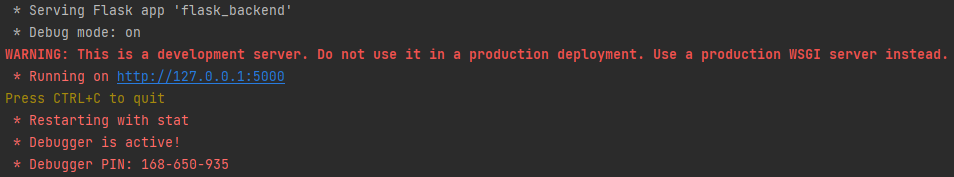
\includegraphics[width=\linewidth]{images/anexoA/server.png}
    \caption*{Figura: Salida tras la ejecución del servidor}
\end{figure}

Esto permite saber que el servidor se encuentra en funcionamiento, y por lo cual que se puede acceder a la herramienta de una de las siguientes formas:
\begin{itemize}
    \item Haciendo click sobre la dirección IP que aparece en dicha salida. Esto abrirá la herramienta en una nueva pestaña del navegador por defecto.
    \item Accediendo a \href{localhost:5000/}{localhost:5000/} en un navegador.
\end{itemize}

Como la herramienta funciona como cliente/servidor, donde el navegador funciona como cliente y Python funciona como servidor, si se detiene la ejecución del fichero \emph{flask\_backend.py}, la herramienta dejará de funcionar.

\section*{Elementos en común}
\addcontentsline{toc}{section}{Elementos en común}

Todas las páginas tiene algunos elementos en común, por lo que en lugar de repetirnos y explicarlos en cada sección, se desarrollan a continuación.

Para saber a qué nos referimos, se incluye la \autoref{im:proveSD} con una página cualquiera que se usará como ejemplo para explicar estos elementos.
\begin{figure}[H]
    \centering
    \fbox{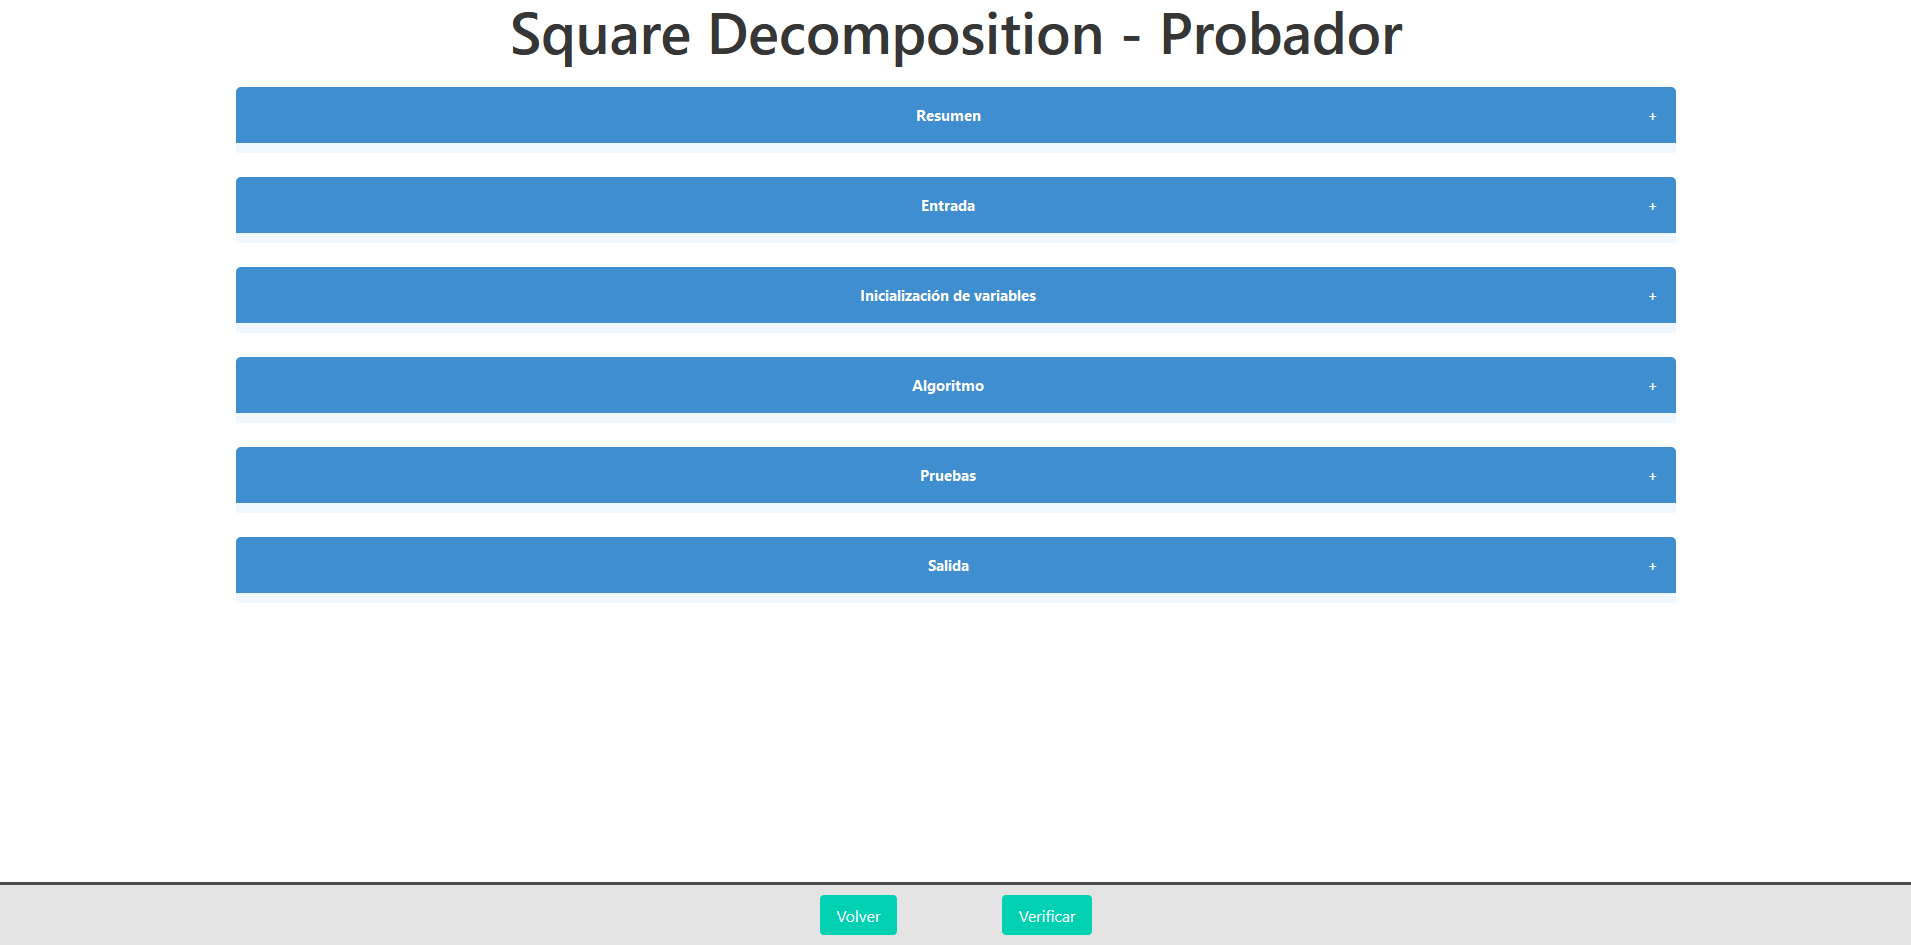
\includegraphics[width=\linewidth]{images/anexoA/probadorSD.png}}
    \caption{Página de la prueba de la Descomposición Cuadrada}
    \label{im:proveSD}
\end{figure}

Como se puede ver en la \autoref{im:proveSD}, lo primero que hay en la página es el título indicando qué se está realizando en dicha página. Por ejemplo, en esta página se muestra el algoritmo que realiza el probador al usar el algoritmo \emph{Square Decomposition}.

Luego, el cuerpo de la página está formado por distintas cajas de color azul con un texto en medio. Este texto indica que se realiza o que datos se muestran en dicha caja. Por ejemplo, la caja con el nombre ``Resumen'' contiene un breve resumen del funcionamiento del algoritmo, mientras que la caja ``Entrada'' contiene la lista de valores que el algoritmo toma como entrada. Para ver el contenido de la caja, únicamente hay que hacer click sobre ella, lo cuál provocará que se expanda mostrando el contenido de la misma. Haciendo otro click, la caja volverá a cerrarse ocultando el contenido y permitiendo así centrarnos en la parte que nos interesa, sin necesidad de ver el contenido de otras cajas que puedan ser una distracción. La única diferencia a esta regla son en el resultado de las verificaciones, cuya caja se mostrará extendida por defecto.

Por ejemplo, el contenido de la página de la figura anterior con alguna caja extendidas es el de la \autoref{im:proveSD_extended}.
\begin{figure}[H]
    \centering
    \fbox{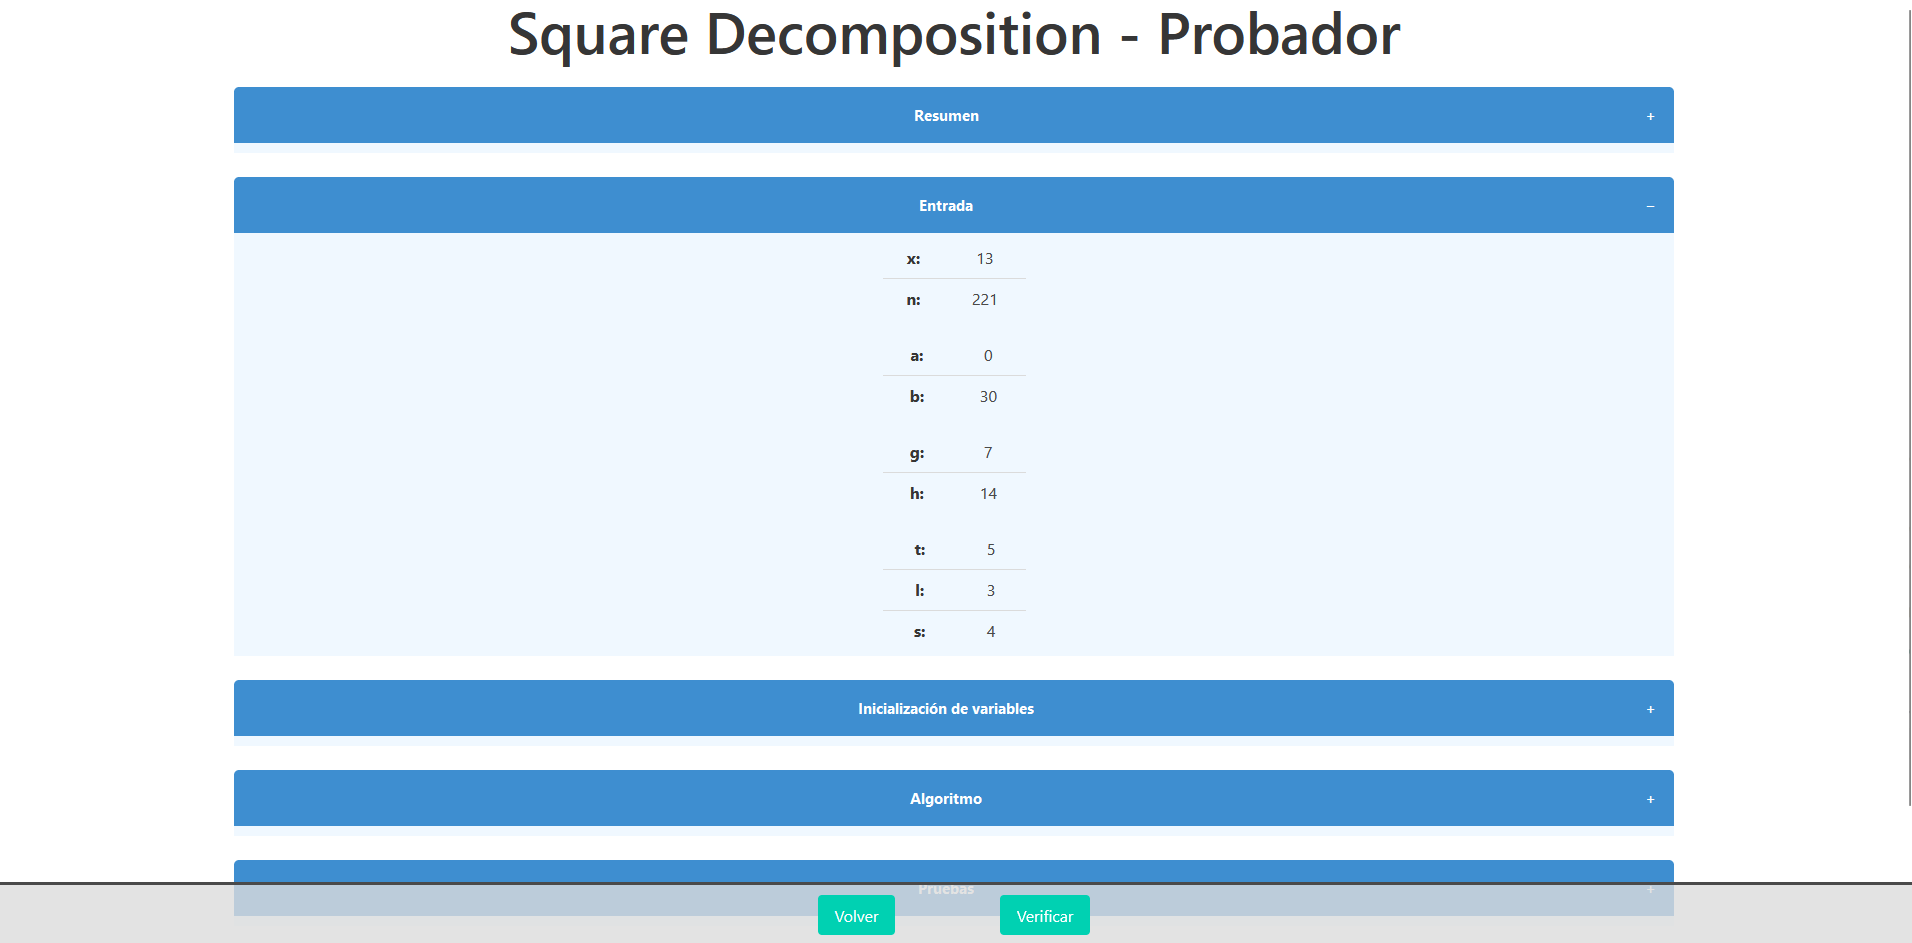
\includegraphics[width=\linewidth]{images/anexoA/probadorSD_extendido.png}}
    \caption{Página de la prueba de la Descomposición Cuadrada}
    \label{im:proveSD_extended}
\end{figure}
En la \autoref{im:proveSD_extended} se puede ver como se ha extendido la caja con los valores de la entrada. Esto provoca que el resto de cajas que se encuentran debajo se desplacen para dejar el espacio suficiente. Además, en caso de no entrar en la página, como ocurre en la imagen, aparecerá una barra lateral que nos permitirá desplazarnos hacia arriba o hacia abajo en la página.

Otro elemento que tienen en común en todas las páginas es la barra inferior. Esta barra contendrá uno o varios botones dependiendo de la página en la que nos encontremos, y siempre se encontrará anclada al borde inferior de la página encima de los demás elementos de la página.

En todas las páginas menos en la página inicial hay un botón para volver a la página anterior. En el caso de que haya una página a la que sea posible acceder desde varias distintas, nos devolverá a la que hayamos usado para acceder.

Además, en todas las páginas en las que se incluya una prueba, también habrá un botón para acceder a la página que contiene la verificación de dicha prueba.

\section*{Inicio}
\addcontentsline{toc}{section}{Inicio}

Al iniciar la herramienta, la primera página a la que se accede es la siguiente:
\begin{figure}[H]
    \centering
    \fbox{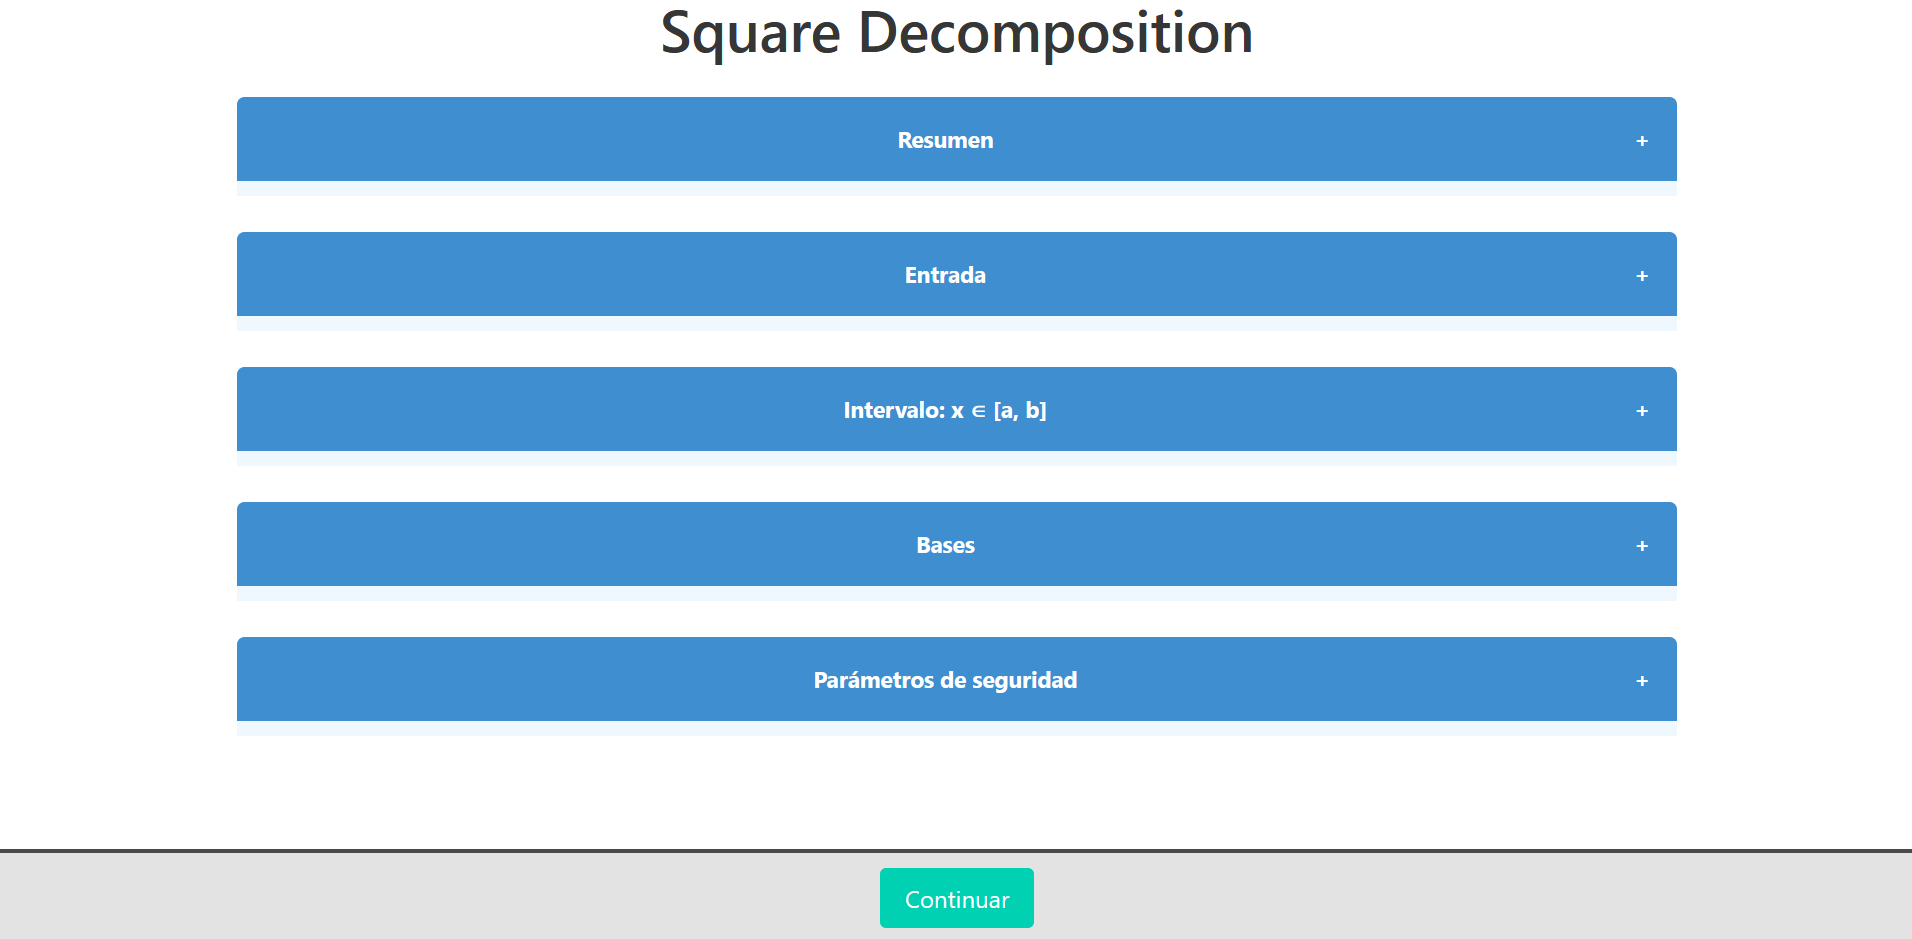
\includegraphics[width=\linewidth]{images/anexoA/input.png}}
    \caption{Página de inicio}
    \label{im:input}
\end{figure}

Esta página sirve para poder indicarle los valores que tomará el algoritmo, divididos en las siguientes entradas:
\begin{itemize}
    \item Entrada: Tiene las siguientes entradas:
    \begin{itemize}
        \item $x$: Valor del secreto.
        \item $n$: Valor del módulo, es decir, el algoritmo utilizará el anillo $\mathbb{Z}_{n}$.
    \end{itemize}
    \item Intervalo: Tiene los siguientes valores del intervalo en el que queremos probar que $x$ pertenece:
    \begin{itemize}
        \item $a$: Valor inferior del intervalo.
        \item $b$: Valor superior del intervalo.
    \end{itemize}
    \item Bases: Tiene las entradas de las bases del algoritmo:
    \begin{itemize}
        \item $g$.
        \item $h$: Tiene que estar generada por $g$ en $\mathbb{Z}_{n}$.
    \end{itemize}
    \item Parámetros de seguridad: Contiene las entradas de los parámetros de seguridad a usar:
    \begin{itemize}
        \item $t$.
        \item $\ell$.
        \item $s$.
    \end{itemize}
\end{itemize}

Las entradas son de la siguiente forma:
\begin{figure}[H]
    \centering
    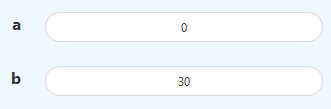
\includegraphics[width=0.5\linewidth]{images/anexoA/input_box.png}
    \captionsetup{labelformat=empty}
    \caption{Ejemplo de campo de entrada}
    \label{im:input_box}
\end{figure}

Donde el texto que hay a la izquierda es el nombre de la entrada, que será uno de los indicados previamente, y la caja que hay a la derecha sirve para entrar el valor deseado. Para introducir un valor, simplemente hay que hacer click sobre la caja correspondiente, lo cuál nos permitirá modificarla leyendo los valores introducidos con el teclado.

Para poder ejecutar la herramienta de manera más rápida, todas las cajas están inicializadas con un valor por defecto que puede ser modificado en el fichero \emph{input.html}.

Al pulsar el botón ``Continuar'' en el menú inferior, la herramienta leerá todos los valores introducidos y hará una serie de comprobaciones, como que ambos extremos del intervalo sean menores que el valor del módulo, que la cota inferior sea menor que la cota superior del intervalo, y que el secreto pertenezca al intervalo. Si alguna de estas comprobaciones falla, aparecerá un mensaje por pantalla indicando el error para que pueda ser solucionado. Si todas las comprobaciones son correctas, redigirá hacia la siguiente página, que contiene los resultados de la prueba.

\section*{Pruebas}
\addcontentsline{toc}{section}{Pruebas}

En esta sección se detalla el funcionamiento de cuatro páginas, que sirven para las pruebas de los distintos algoritmos usados, ya que todas ellas tienen un funcionamiento. Estas son la prueba del algoritmo \nameref{alg:prove wt}, la \nameref{alg:prove s}, la \nameref{alg:prove ss} y la \nameref{alg:prove li}.

Para ello se verá en detalle la primera de ellas, y se comentaran las diferencias que incluyen las demás. La página para esta prueba es la siguiente:
\begin{figure}[H]
    \centering
    \fbox{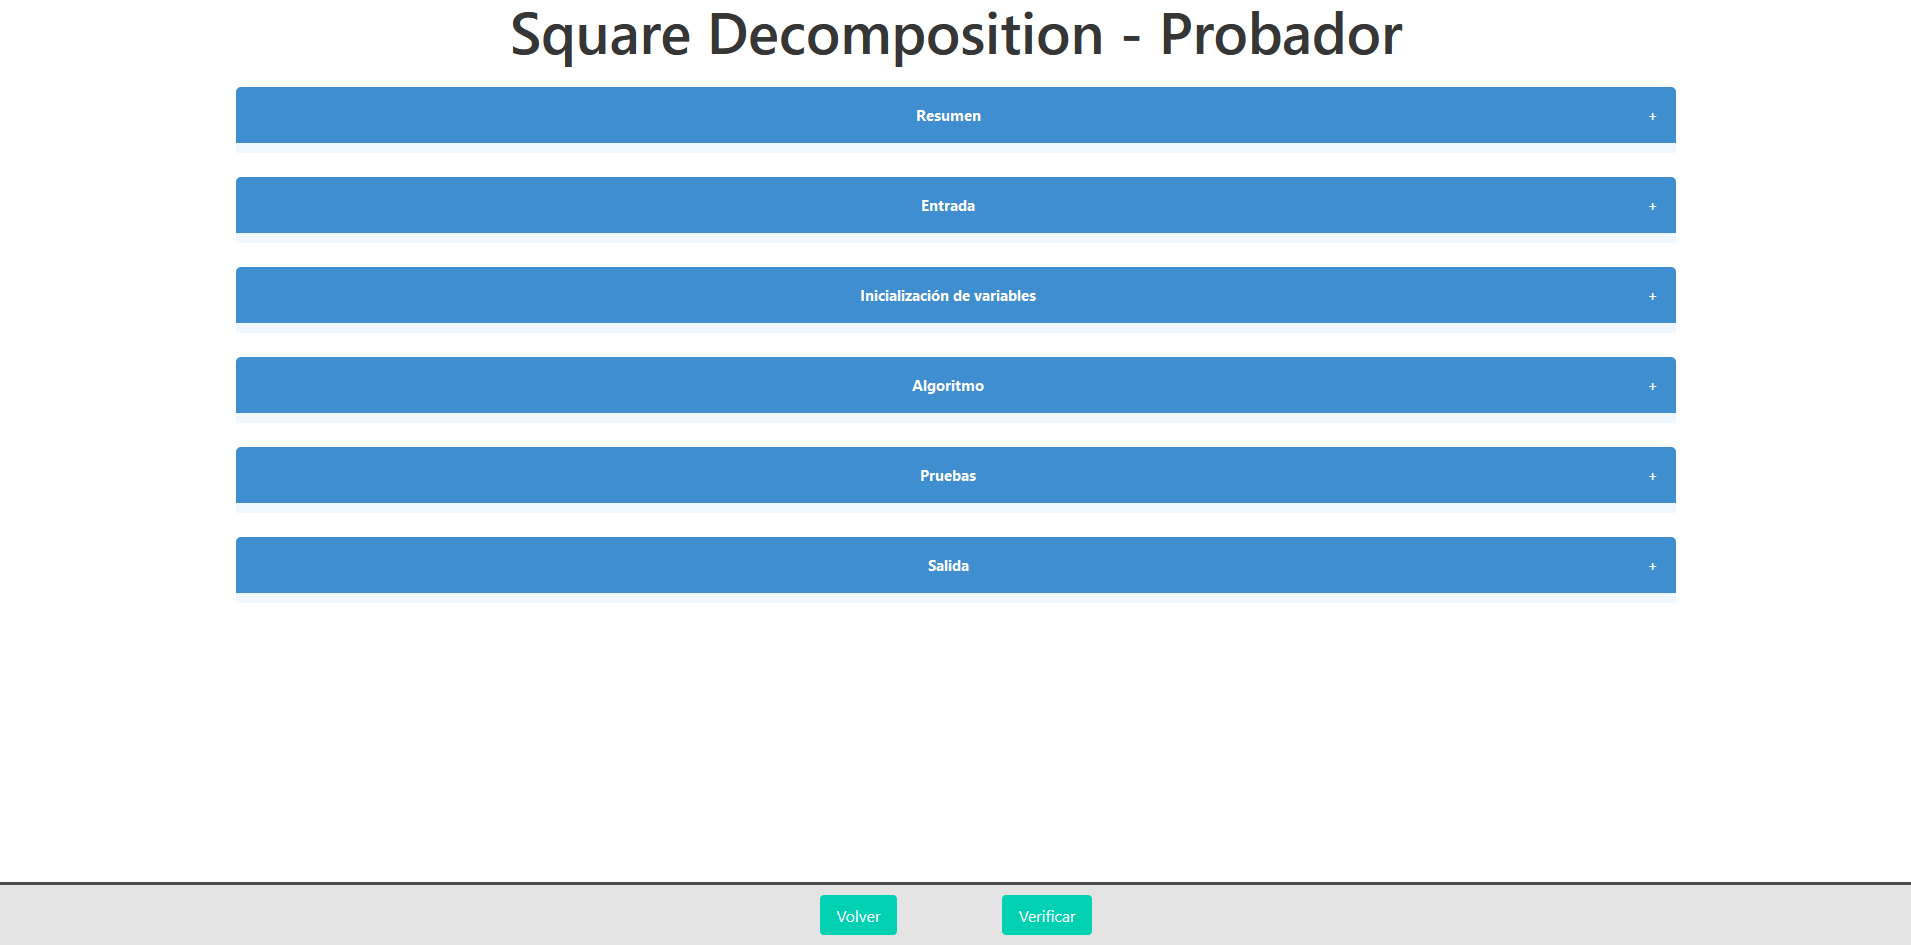
\includegraphics[width=\linewidth]{images/anexoA/probadorSD.png}}
    \caption{Página de la prueba de la Descomposición Cuadrada}
    \label{im:proveSD2}
\end{figure}

Las distintas partes que incluyen son:
\begin{itemize}
    \item Resumen. Aquí se hace un breve resumen del funcionamiento del algoritmo. Sin embargo, no tiene la intención de detallar su funcionamiento, lo cuál se hace en el \nameref{sec:teoria}.

    \item Entrada. Contiene una lista con todos los valores que toma el algoritmo como entrada, que en el caso del ejemplo, en la prueba de la \emph{Descomposición Cuadrada} será los que se hayan introducido en la página anterior, y en las demás pruebas serán los correspondientes según el algoritmo.

    \item Inicialización de variables. Esta parte es exclusiva de la prueba de la \emph{Descomposición Cuadrada}. Antes del algoritmo, hay algunas variables que se inicializan de forma aleatoria, que se detallan en esta caja.

    \item Algoritmo. Se muestra la ejecución del algoritmo, incluyendo tanto las expresiones con el nombre de las variables como con los valores de la ejecución realizada. Con esto, se puede seguir fácilmente el algoritmo, sabiendo de dónde proceden los valores utilizados en el algoritmo.

    \item Pruebas. En el caso de que la prueba utilice otro algoritmo, se incluye botones para acceder a la página de dicha prueba. Esto ocurre en la prueba del algoritmo \nameref{alg:prove wt}, que incluye botones a la \nameref{alg:prove s} y a la \nameref{alg:prove li}; y en el caso de la \nameref{alg:prove s}, que incluye botones a la \nameref{alg:prove ss}.

    En las otras pruebas, estos campos no existen.

    \item Salida. Aquí se muestra una lista con los valores obtenidos tras la ejecución del algoritmo. En el caso de la prueba de la \emph{Descomposición Cuadrada}, la mayoría de estos valores se pueden modificar para forzar así que la prueba sea incorrecta, lo cuál permite ver como la verificación puede rechazar la prueba.

    En el caso de que se modifique estas salidas, sobrescribirán los valores que se tenían previamente al pulsar cualquier botón que nos redirija a otra página, por lo que si queremos volver a obtener la prueba correcta será necesario volver a la página de inicio y volver a introducir los valores.
\end{itemize}

\section*{Verificaciones}
\addcontentsline{toc}{section}{Verificaciones}

Igual que en la sección anterior con las pruebas, a continuación se desarrollan todas las verificaciones en la misma sección. Esto incluye las verificaciones de \nameref{alg:verify wt}, de la \nameref{alg:verify s}, de la \nameref{alg:verify ss} y de la \nameref{alg:verify li}.

De nuevo, se usará la verificación de la primera de ellas como ejemplo, y se comentarán las diferencias que existan en las demás:
\begin{figure}[H]
    \centering
    \fbox{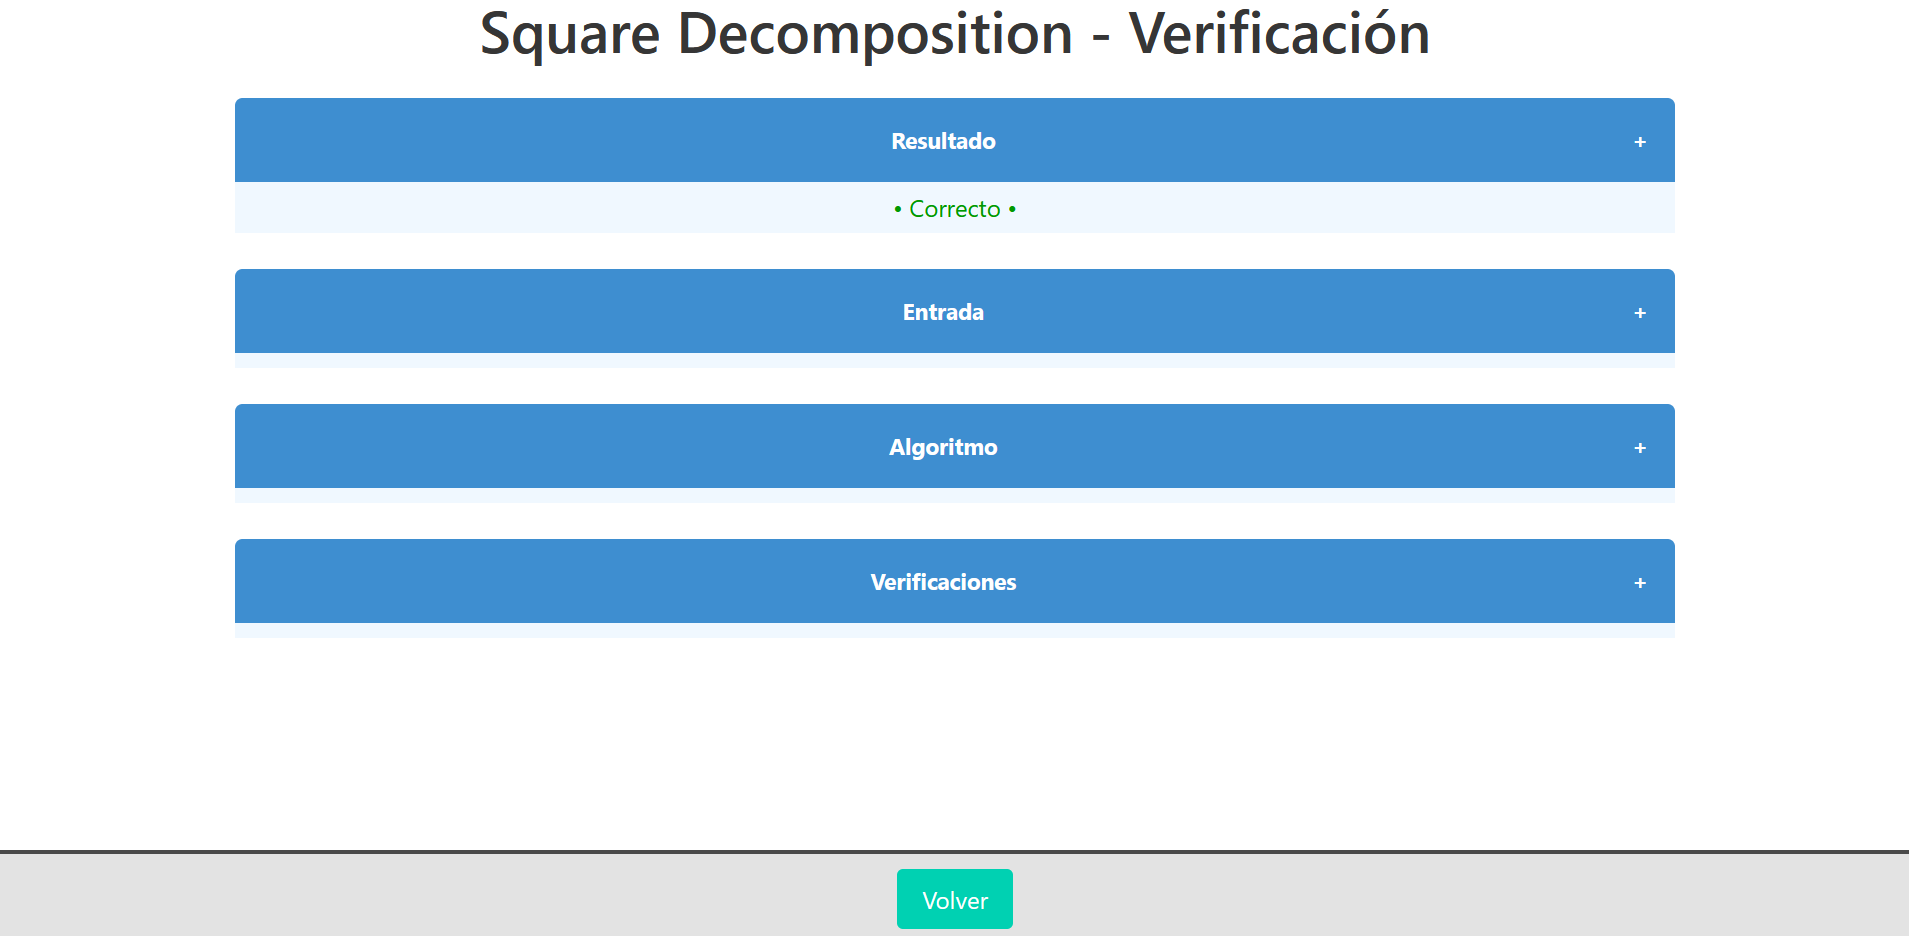
\includegraphics[width=\linewidth]{images/anexoA/verifySD.png}}
    \caption{Página de la verificación de la Descomposición Cuadrada}
    \label{im:verifySD}
\end{figure}

Los campos que incluyen son:
\begin{itemize}
    \item Resultado. Esta es la única caja que por defecto está expandida, para una mayor comodidad a la hora de comprobar los resultados. Contiene los resultados de la verificación, que puede ser correcta (en cuyo caso aparecerá en verde) o incorrecta (en cuyo caso aparecerá en rojo).

    \item Entrada. Contiene una lista con los valores que el algoritmo toma como entrada, que coincidirá en gran medida con la salida de la prueba correspondiente.

    \item Algoritmo. Igual en las pruebas, se incluye el funcionamiento paso por paso de la verificación, incluyendo tanto las fórmulas con los nombres de las variables como los valores de esta ejecución.

    \item Verificaciones. En caso de que la verificación requiera de otro algoritmo de verificación, se incluirá un botón en esta caja para acceder a la página de dicha verificación. Esto ocurre en el caso de la verificación de \nameref{alg:verify wt}, que requiere las verificaciones de la \nameref{alg:verify s} y de la \nameref{alg:verify li}; y en la verificación de la \nameref{alg:verify s} que requiere la verifiación de la \nameref{alg:verify ss}.
\end{itemize}